
%%%%%%%%%%%%%%%%%%%%%%%%%%%%%%%%%%%%%%%%%%%%%%%%%%%%%%%%%%%%%%%%%%%%%%%%%%%%%%%%%%%%%%%%%%%%%%%%%%%%%%%%%%%%%%
% Article:
% Bootstrap Inference for the Area Under the ROC Curve
% Solution
%%%%%%%%%%%%%%%%%%%%%%%%%%%%%%%%%%%%%%%%%%%%%%%%%%%%%%%%%%%%%%%%%%%%%%%%%%%%%%%%%%%%%%%%%%%%%%%%%%%%%%%%%%%%%%%


% \section{Statistical Methodology} \label{sec:theory}
% \section{Statistical Methodology} \label{sec:theory}


\section{The Optimization Problem} \label{sec:theory}



% \textbf{Introduction: Solution approach}

A distribution could shift in a number of directions, a given distance from the reference distribution.
For many shifts likely to occur, the AUROC may change little, while for some deviations in particular directions, the AUROC could show an extreme change.
The most conservative solution, from the forecasters perspective, is the most extreme values that can be reached by shifting the distribution a specified distance.

%Procedure and motivation:
%\begin{itemize}
%    \item Existing literature seeks to characterize variability due to \emph{sampling variation}
%    \item In this paper, I allow for additional variation in the sample due to changes in the underlying distribution
%    \item How far would the AUROC move before model rebuild is triggered?
%\end{itemize}

%{\Large: Can I find a way to explain this:}
%To demonstrate this, I could plot a set of level curves, showing the deviation in an intuitive direction with that in the optimized direction.
%It would be a set of ovals, with large shifts possible for given distances, and moderate shifts possible for common changes (such as a change in mean of the positive scores).
%\textbf{Give more thought to the axes.}

\subsection{Optimization Problem: Extreme Values of AUROC}

% State original optimization problem.
The solution of the desired bounds of the prediction interval is the distribution that satisfies the following optimization problem.
Suppose that classification variables for positive observations have marginal distribution $f$ and those for negative observations have marginal distribution $g$.
Together, these have a joint distribution with weights defined by the product $\mathbf{f} \otimes \mathbf{g}$, when discretized and expressed in vector form.
%
To find the upper bound of the prediction interval, $A^{(U)}$, this optimization problem is
%
\begin{equation}
    \max_{\mathbf{u}, \mathbf{v}} \frac{1}{m n} \sum_{i = 1}^{m} \sum_{j = 1}^{n} u_i v_j I_{\left\{ y_j > x_i \right\}}
\end{equation}
%
\noindent subject to
\begin{align}
    D(\mathbf{u} \otimes \mathbf{v}, \mathbf{f} \otimes \mathbf{g}) \leq \bar{D} \\
    %
    \sum_{i = 1}^{m} u_i = 1, \quad \sum_{j = 1}^{n} v_j = 1 \\
    %
    \left\{ u_i  \geq 0 \right\}_{i=1}^{m}, \quad \left\{ v_j \geq 0 \right\}_{j=1}^{n}.
    %
\end{align}
%
\noindent The objective function is the expression for the area under the ROC curve as it would be calculated if the sample had classification variables of $y$, with distribution $u$, and $x$, with distribution $v$.
Together, these have a joint distribution with weights defined by the product $\mathbf{u} \otimes \mathbf{v}$.
The first condition constrains the distribution of the joint densities $\mathbf{u} \otimes \mathbf{v}$ and $\mathbf{f} \otimes \mathbf{g}$ to differ by the specified distance $\bar{D}$.
%
The remaining conditions specify that the distributions are well-defined.
%
The corresponding minimization problem results in the lower bound of $A^{(L)}$. 
% 
Where the distance function $D(\cdot)$ is Kullback-Leibler divergence, this problem is equivalent to finding the highest value $A^{(U)}$ and lowest value $A^{(L)}$ such that the relative entropy is within an allowable level $\bar{D}$. 


\subsection{Dual Problem: Distance to a Distribution with AUROC $A_0$}

There is, however, an indirect method of solving this problem.
This is because an increase in distance allows for a larger choice set, so there is the potential for finding more extreme values of $A^{(L)}$ and  $A^{(U)}$ with an increase in $\bar{D}$.
%
% \textbf{Monotonicity:}
%
There is a weakly monotonic relationship between optimized distance in $A_0$-space and distance in distribution space.
% Clearly (ding!), increasing available distance increases choice set for further $A_0$ values, so you can always do weakly better, in terms of further away.
While the original problem is to maximize distance in $A_0$-space, subject to a constraint on the distance allowed,
the dual problem is to minimize distance in the space of distributions, subject to a constraint on the candidate AUROC.



% \textbf{Specification of Optimization Problem}

Find the \emph{minimum} distance from the observed distribution and a distribution that has a particular value of the AUROC.
%
\begin{equation}
    \min_{\mathbf{u}, \mathbf{v}}
        D(\mathbf{u} \otimes \mathbf{v}, \mathbf{f} \otimes \mathbf{g})
\end{equation}
%
\noindent subject to
%
\begin{align}
    \frac{1}{m n} \sum_{i = 1}^{m} \sum_{j = 1}^{n} u_i v_j I_{\left\{ y_j > x_i \right\}} \geq A^{(U)}_0 \\
    %
    \sum_{i = 1}^{m} u_i = 1, \quad \sum_{j = 1}^{n} v_j = 1 \\
    %
    \left\{ u_i  \geq 0 \right\}_{i=1}^{m}, \quad \left\{ v_j \geq 0 \right\}_{j=1}^{n}.
    %
\end{align}
%
% Under this specification of the problem, the solution is a distribution 
Where the distance function $D(\cdot)$ is Kullback-Leibler divergence, this problem is equivalent to finding the distribution with minimum differential entropy among those with AUROC statistics no smaller than the candidate value of $A^{(U)}_0$. 



%\begin{itemize}
%    % \item $\min_{\mathbf{u},\mathbf{v}}
%    %     D(\mathbf{u},\mathbf{f}, \mathbf{v},\mathbf{g})$
%    \item subject to
%    $\frac{1}{m n} \sum_{i = 1}^{m} \sum_{j = 1}^{n} u_i v_j I_{\left\{ y_j > x_i \right\}} = A_0$,
%    \item unit mass constraints
%    $\sum_{i = 1}^{m} u_i = 1, \quad \sum_{j = 1}^{n} v_j = 1$,
%    \item nonnegativity constraints
%    $ \left\{ u_i  \geq 0 \right\}_{i=1}^{m}, \quad \left\{ v_j \geq 0 \right\}_{j=1}^{n}$
%    \item where $\mathbf{f}$ and $\mathbf{g}$ are the observed distributions of classification variables for positive and negative cases, respectively,
%    while $\mathbf{u}$ and $\mathbf{v}$ are the closest weights that satisfy $A = A_0$
%\end{itemize}



% \textbf{Solution}

The solution can be stated in terms of the derivatives of the distance functions with respect to the optimized distribution weights.
%
This solution results in first order conditions
\begin{align}
    %
    \frac{d D(\mathbf{u},\mathbf{f})}{d u_i} = \lambda \sum_{j = 1}^{n} v_j I_{\left\{ y_j > x_i \right\}} + \gamma_x + \delta_{x,i},
    i = 1, \dots, m \\
    %
    \frac{d D(\mathbf{v},\mathbf{g})}{d v_j} = \lambda \sum_{i = 1}^{m} u_i I_{\left\{ y_j > x_i \right\}} + \gamma_y + \delta_{y,i},
    j = 1, \dots, n.
    %
\end{align}
%
That is, the change in distance is equal to a partial AUROC term plus some extra terms for the Lagrange multipliers on the remaining constraints. Exactly how this is satisfied depends on the particular choice of distance function $D(\mathbf{u} \otimes \mathbf{v}, \mathbf{f} \otimes \mathbf{g})$.





\subsection{Specification of Distance}


A distance function $D(\cdot)$ must be specified for calculating the distance to the distributions for calculation of the bounds on AUROC.
%
%
The recommended metric is Kullback-Leibler divergence (KLD), first presented in \citet{kullbackliebler1951}.
%
The original specification is not technically a distance metric, since it is not symmetric, but 
% 
it still specifies a useful criterion for discriminating between distributions:
% 
% \citet{bigi2003chapter} highlights a symmetric version.
%
% In both versions, it is used as a criterion for discriminating between distributions:
% 
% 
%%%%%%%%%%%%%%%%
% {\Large Don't forget to add back the KLD equation}
%%%%%%%%%%%%%%%%
% 
% \begin{equation}
%     KLD_0(f_1, f_2) = \sum_{k = 1}^{K} \left\{ \left( f_1(t_k) - f_2(t_k) \right)
%         \log \left( \frac{f_1(t_k)}{f_2(t_k)} \right) \right\},
% \end{equation}
%
%
\begin{equation}
    KLD_1(h_1, h_2) = \sum_{k = 1}^{K} \left\{ h_1(t_k)
        \log \left( \frac{h_1(t_k)}{h_2(t_k)} \right) \right\}.
\end{equation}
%
% 
\noindent where $h_1$ and $h_2$ are two density functions summed over the index $k = 1, \dots, K = mn$.
In the objective functions of the optimization problems above, these functions are the joint densities
$\mathbf{f} \otimes \mathbf{g}$ and $\mathbf{u} \otimes \mathbf{v}$, before and after optimization.
In the first order conditions, the derivatives of this function have the pairs of distributions set at either
$\mathbf{g}$ and $\mathbf{v}$ or $\mathbf{f}$ and $\mathbf{u}$,
for the positive and negative classification variables, respectively.

With a single density term in the equation, it is implied that the distribution $f_1$ is a benchmark distribution, or null hypothesized distribution, under which the true probabilities are calculated.
The same logic applies to the differential weighting on low density areas of the support, so it is also a good candidate for the specification of distance in the optimization problem.



\input{Figs/KLD/FigsKLDdist1.tex}

\citet{bigi2003chapter} highlights a symmetric version of this criterion, which is useful for explaining the suitability of such a measure of distance.
%
\begin{equation}
    KLD_2(h_1, h_2) = \sum_{k = 1}^{K} \left\{ \left( h_1(t_k) - h_2(t_k) \right)
        \log \left( \frac{h_1(t_k)}{h_2(t_k)} \right) \right\}.
\end{equation}
%
% 
As seen in Figure \ref{fig:KLDdistance1} above, the log-distance term takes on much more extreme values, particularly in areas where one of the distributions has low density.
This is because $KLD_2(\cdot)$ is designed as a means of discriminating between two distributions.
When there is an observation that occurs in a region of the support where there is very low density in one distribution and very high density in the other, there is very strong support for the hypothesis that it came from the second distribution.
In the extreme case when the supports of the distributions do not overlap, there is perfect ability to discriminate between the distributions.

This feature is also useful in the sense that it will place more weight on the changes in density that are more closely related to changes in AUROC.
This is concentrated in the region between the two distributions of classification variables, particularly when only the tails overlap.
In this case, comparatively large changes can be made in terms of AUROC with marginal changes in densities.

% The same is true of the asymmetric version of this statistic, denoted $KLD_1()$, which takes on the following form.






% Why Kullback-Leibler Divergence?
There are several good reasons to choose either of these functions as the measure of distance.
%
First of all, there is an information-theoretic justification.
It adequately measures the quality of information for discriminating between pairs of distributions.
Secondly, it also plays a role in the derivation of the distribution theory for the maximum likelihood estimator (see \citet{amemiya1985}, for example).
In some versions of this derivation, the distribution is made up of two important terms.
The first of which measures the information from the true distribution from which the sample is drawn.
This is defined as the expected value of the log of the density, a quantity that is also defined in \citet{kullbackliebler1951}.
This is fixed relative to the fitted distribution and any parameters that may appear in a maximum likelihood estimation procedure.
The second term is the $KLD_1$ function evaluated at the fitted distribution and the true distribution.
Thus, the $KLD_1$ metric is the first order term in the distribution of the fitted model from the true distribution in a maximum likelihood framework.
%
This extends the applicability to any situation in which the researcher could specify a distribution and estimate its variability by maximum likelihood.

%\begin{itemize}
%    \item Information-theoretic justification: Measures quality of information for discriminating between pairs of distributions
%    \item Relation to MLE: $KLD(f_1, f_2)$ is the second term in the asymptotic distribution of the MLE (the first is the information from $f_1$), where $f_2$ is the distribution fitted to data from true distribution $f_1$
%    \item More weight on tails: Penalty for deviations in low density has more influence on variation of AUROC, since the variation in AUROC is generated where the densities overlap
%\end{itemize}

% Refer to remainder terms in \citet{amemiya1985} when deriving the distribution of the distance.




% \textbf{Why not $\chi^2$?}

Still, one may put forth the suggestion that the modeling could be simplified by the use of a $\chi^2$ calculation instead, such as
%
% Another option is a chi-square approach as in \citet{chernofflehmann1954} (which also shows that it works for binned data but not empirical distributions).
%
% \begin{equation}
%     CHI(f_1, f_2) = \sum_{k = 1}^{K} \left( f_1(t_k) - f_2(t_k) \right)^2.
% \end{equation}
%
the sum of the squared differences between the two joint density functions on the grid $k = 1, \dots, K$.
% 
This specification has the drawback of assigning equal weight on equal deviations at all points in the distribution.
For discriminating between distributions, this is not ideal, since it places undue weight on dense regions where a small difference is less likely to be informative.
%
Aside from the conceptual advantage, this option suffers from a computational drawback.
Computationally, this specification of distance requires additional constraints to impose non-negativity of densities when shifting distributions toward the limits of AUROC.
The $KLD$ metric guarantees an interior solution, which is the subject of the next section.

%\begin{itemize}
%    \item Equal weight on equal deviations at all points in the distribution
%    \item Overlapping tails of distributions is where discriminating power is greatest
%    \item Computationally, requires additional constraints to impose non-negativity of densities when shifting distributions
%\end{itemize}




% One is simple and leads to a linear updating rule, except that it does not automatically enforce nonnegativity of the probabilities, which must be imposed by constraint.

% The recommended requires nonlinear optimization but self-imposes nonnegativity.


% \subsection{Solution and Algorithm}
\subsection{Solution}

% First order conditions, see appendix for derivation.
While a more complete listing of the calculations is offered in \ref{app:soln}, the solution to the distance minimization problem, with $KLD_1$ as the chosen distance metric, is represented by
%
\begin{align}
    %
    u_i = \exp{ \left\{ 1 + \ln f_i + u_i \ln f_i
        + \lambda \sum_{j = 1}^{n} v_j I_{\left\{ y_j > x_i \right\}} + \gamma_x \right\} } \\
        %
    v_j = \exp{ \left\{ 1 + \ln g_j + v_j \ln g_j
        + \lambda \sum_{i = 1}^{m} u_i I_{\left\{ y_j > x_i \right\}} + \gamma_y \right\} }
        %
\end{align}

\noindent where $k_x$ and $k_y$ are normalizing constants and Lagrange multiplier $\lambda$ is the step size.

% Describe switching algorithm.
%
This nonlinear system of equations has a large number of parameters and would be difficult to solve explicitly.
%
Instead, this system of equations is solved via a switching algorithm with the recurrence relations
%
\begin{align}
%
    u_i^{(t+1)} = k_x f_i ^{1 + u_i^{(t)}}
            \exp{ \left\{ \lambda \sum_{j = 1}^{n} v_j^{(t)} I_{\left\{ y_j > x_i \right\}} \right\} } \\
%
    v_j^{(t+1)} = k_y g_j ^{1 + v_j^{(t)}}
            \exp{ \left\{ \lambda \sum_{i = 1}^{m} u_i^{(t)} I_{\left\{ y_j > x_i \right\}}  \right\} }
%
\end{align}
%
\noindent A switching solution is effective, since the main terms in the recurrence relations are the cross-partial-AUROC expressions represented by, for example, $\sum_{j = 1}^{n} v_j^{(t)} I_{\left\{ y_j > x_i \right\}}$.
%
These terms specify the direction toward the optimal distribution and the Lagrange multiplier $\lambda$ specifies the step size.
The log operators in the distance function enforce an interior solution, so the non-negativity constraints are automatically satisfied.
At each step, the constants $k_x$ and $k_y$ serve to normalize to unit probability mass.

%
%\begin{itemize}
%    \item[1] Build model from entire sample and measure AUROC
%    \item[2] Measure distance between distributions in a series of subsamples
%    \item[3] Calculate extreme AUROC values that correspond to movements away from full dataset, using distances between observed distributions
%\end{itemize}



% \subsection{Prediction Intervals} % \label{sec:conf}
\subsection{Forecast Intervals} % \label{sec:conf}

% \textbf{Prediction Intervals $[A_L, A_U]$}

%Solving for extreme values of $A$ for a particular distance $\bar{D}$
%\begin{itemize}
%    \item Record estimate of AUROC, $\hat{A}$
%    \item Solve distance minimization problem for a particular $A_0$
%    \item Search on $A_0$ above $\hat{A}$ until $\hat{D} = \bar{D}$ $(\rightarrow A_U)$
%    \item Repeat for $A_0$ below $\hat{A}$ $(\rightarrow A_L)$
%\end{itemize}


The solution of this problem allows for the calculation of the bounds of the forecast interval.
% Method of calculation:
First, use the classification variables from the entire
% 
\footnote{In practice, a modeler may choose a specific sample deemed appropriate for estimation of a model. This will often not be the full sample of all available observations, as the modeler would take into account the features of a sample to best represent the anticipated scenarios in future uses of the model. 
This sample will often be combined with several validation samples, representing a variety of situations that could be encountered through the use of the model but these would typically be used as a form of stress test and not as a benchmark for model performance. 
Thus, these would be left out of the sample for estimating the reference AUROC value from which the forecast interval is constructed. }
% 
build sample and measure the AUROC, $\hat{A}$.
%
Next, measure the distance $\bar{D}$ between the distributions
%
through some modeling approach.
%
This is facilitated if the researcher has some knowledge of how to model the variation in the distribution.
In particular, a maximum likelihood approach could be used to model this variation.
%
This can be achieved if the modeler has a specific model in mind.
%
However, it could also be achieved as long as the sample can be divided into several segments with known differences, such as seasonality.
%
Then, the variation in distributions could be calculated
in a series of subsamples from the empirical distribution defined by the full sample.
%
Of course, in order to calculate $\bar{D}$ using this approach,
%
it is necessary that the modeler is aware of a segmentation of the sample into sections that will indicate the appropriate distance.
%
Another approach would be to re-sample from the full distribution and calculate a bootstrap version of the distance between subsamples and the full empirical distribution.
%
Take the average of the distances between the distributions and record it as distance $\hat{D}$.
%
Finally, search over the values of $A_0$ both above and below $\hat{A}$ until the distance $\hat{D}$ is achieved, searching in the direction of the partial-AUROC term of the first order conditions above.
%
This is achieved by solving for the distance minimization problem for each candidate value of $A_0$ for bounds $A_L$ and $A_U$,
above and below $\hat{A}$, until $\bar{D} = \hat{D}$ in each direction.
%
% At each candidate value of $A_0$ for bounds $A_L$ and $A_U$, solve the distance minimization problem for that particular $A_0$.
% Search on $A_0$ above and below $\hat{A}$ until $\hat{D} = \bar{D}$ in each direction.





%\subsection{Prediction Intervals} % \label{sec:conf}
%
%\textbf{Prediction Intervals $[A_L, A_U]$}
%
%Solving for extreme values of $A$ for a particular distance $\bar{D}$
%\begin{itemize}
%    \item Record estimate of AUROC, $\hat{A}$
%    \item Solve distance minimization problem for a particular $A_0$
%    \item Search on $A_0$ above $\hat{A}$ until $\hat{D} = \bar{D}$ $(\rightarrow A_U)$
%    \item Repeat for $A_0$ below $\hat{A}$ $(\rightarrow A_L)$
%\end{itemize}



% A prediction interval for the AUROC can be analytically determined by inverting the distance metric, finding the potential AUROC values corresponding to quantiles of the chi-square distribution.
% In each direction, above or below the estimated AUROC, the boundaries of the confidence interval are obtained, such that the distance to the closest distribution with that AUROC is the $1 - \alpha$ quantile of the chi-squared distribution.

% Not required:
% {\Large Show examples from binormal and biexponential model.} Are the confidence intervals symmetric? How do they overlap the theoretical confidence intervals from $z$-statistics? Inside? Outside?

%\textbf{hourglass figure:}
%
%{\Large Insert hourglass figure of AUROC interval possibilities for distributions a specific distance away.}
%Overall, I am measuring the amount of variation that would go undetected by a distance metric from the reference distribution.
%Here, I am showing a continuum of variation, indexed by each particular distance from the reference distribution.
%
%
%
%
%%%%%%%%%%%%%%%%%%%%%%%%%%%%%%%%%%%%%%%%%%%%%%%%%%%%%%%%%%%%%%%%%%%%%%%%%%%%%%%%%%%%%%%%%%%%%%%%%%%%%%%%%%%%%%%


\begin{figure}[h!]

\begin{center}

    \caption{Forecast and Confidence Intervals} \label{fig:Forecast1}

        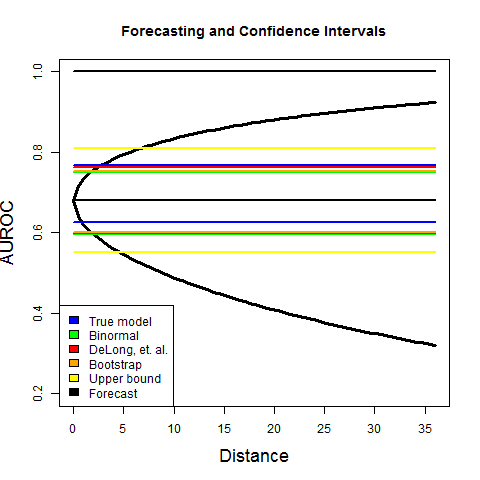
\includegraphics[scale=  0.75]{Figs/Forecast/Forecast_int_1.png}



\end{center}

    \footnotesize

        \textbf{Forecast and Confidence Intervals:}
        Forecast intervals are produced as a function of distance from the sample distribution (black curves).
        Under the null hypothesis of a fixed sampling distribution, distance would follow a $\chi^2$ distribution with $9$ degrees of freedom.
        Confidence intervals are shown for the AUROC for a variety of methods, at the $95\%$ confidence level.
        % 
        As the forecast intervals are scaled by the estimate of distance, it is possible that the intervals will expand to account for added variation, while others remain fixed. 
        %
        The sample is drawn from a bi-normal distribution with a true AUROC of $0.70$, with positive classification variable distribution with a mean of $0$ and standard deviation of $1/\sqrt{2}$, and negative positive classification variable distribution with a mean of $0.5244$ and standard deviation of $1/\sqrt{2}$.
        Sample size is $1,100$ in total, with $1,000$ negative observations and $100$ positive observations.

% Terms in $KLD(\textcolor{blue}{f_1}, \textcolor{red}{f_2})
%  = \sum_{k = 1}^{K} \left\{ \textcolor{magenta}{\big( f_1(t_k) - f_2(t_k) \big)}
%         \textcolor{orange}{\log \left( \frac{f_1(t_k)}{f_2(t_k)} \right)} \right\}$

\end{figure}


%%%%%%%%%%%%%%%%%%%%%%%%%%%%%%%%%%%%%%%%%%%%%%%%%%%%%%%%%%%%%%%%%%%%%%%%%%%%%%%%%%%%%%%%%%%%%%%%%%%%%%%%%%%%%%%


%
%
%
%Forecast intervals as a function of distance from the sample distribution (black curves).
%These are contrasted against a series of $95\%$ confidence intervals for the AUROC for a variety of methods.
%%
%Under the null hypothesis of a fixed sampling distribution, distance would follow a $\chi^2$ distribution with $9$ degrees of freedom.


% \textbf{Regularity Condition (Comparability?):}
% {\Large After solution, show when it exists}

It is important to consider the conditions under which the solution to the above problem exists.
%
The required regularity condition is that the classification variable is not a perfect classifier.
For example, it is sufficient that the support of the positive and negative distributions are not disjoint.
% (actually, sufficient but not necessary) with more than one value in the support (non-singleton).
If so, then one can find a distribution with any AUROC value:
$1$ if all weight of $y$ is on the higher value and all weight of $x$ is on the lower value,
$0$ if all weight of $x$ is on the higher value and all weight of $y$ is on the lower value,
and anything in between for the fractions of weight in between.
% If $3$ obsns in support, there are only more possible permutations.
If there are more values in the support, there are more permutations possible.


%%%%%%%%%%%%%%%%%%%%%%%%%%%%%%%%%%%%%%%%%%%%%%%%%%%%%%%%%%%%%%%%%%%%%%%%%%%%%%%%%%%%%%%%%%%%%%%%%%%%%%%%%%%%%%%
%%%%%%%%%%%%%%%%%%%%%%%%%%%%%%%%%%%%%%%%%%%%%%%%%%%%%%%%%%%%%%%%%%%%%%%%%%%%%%%%%%%%%%%%%%%%%%%%%%%%%%%%%%%%%%%
